\begin{figure}

\centering
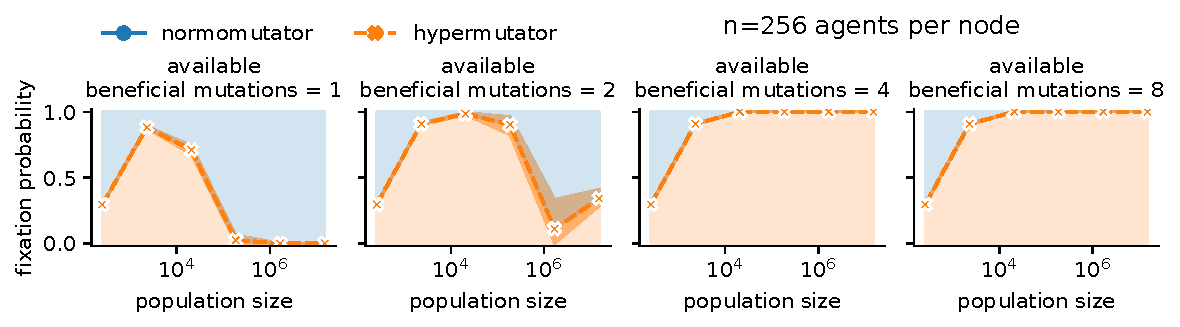
\includegraphics[width=0.8\linewidth]{binder/binder-wse-5050-spatial2d-2048atile-traits.ipynb/binder/teeplots/wse-5050-spatial2d-2048atile-traits/col=available-beneficial-mutations+errorbar=ci+hue=genotype+style=genotype+viz=size-fixation-areaplot+x=population-size+y=fixation-probability+ext=.pdf}%
\vspace{-3ex}
\caption{
\textbf{Restricted adaptive potential favors nonmutators.}
\footnotesize
Area plots show fixation probabilities in WSE simulations initialized with even mix of mutator and nonmutator genotypes.
As available beneficial mutations increase, mutattors gain favor in progressively larger populations.
% Simulations were conducted on WSE using the counter-based genome model, with populations initialized to a 50/50 mix of non- and mutators.
% Subpopulations comprised 2,048 agents per PE.
Shaded bands show bootstrapped 95\% confidence intervals.
% Supplementary Figure \ref{fig:fixheat-wse-altatile:2048} details results in a tabular format.
}
\label{fig:avail-ben-muts}

\vspace{-3ex}

\end{figure}
